% Chapter 3

\chapter{Extrapolating average accuracy} % Main chapter title

\newcommand{\skone}{\mathcal{S}_{k_1}}
\newcommand{\sktwo}{\mathcal{S}_{k_2}}


\label{Chapter3} % For referencing the chapter elsewhere, use \ref{Chapter1} 

\section{Introduction}

In this chapter, we address the question of how to estimate the
$k$-class average risk, $\text{AvRisk}_{k, r}$, based on data from a
problem $P_1$ with $k_1 < k$ classes, and $r = r_1$-repeat training
data.  We continue with the framework introduced in Chapter 2,
including the definition of the average risk and the marginal property
of classifiers.  However, we generalize the cost function $C(y;
\hat{y})$ from the zero-one cost function to a general nonnegative cost function.

We begin by continuing to analyze the average risk $\text{AvRisk}_{k,
  r}$, which results in an explicit formula for the average risk.  The
formula reveals that all of the information needed to compute the
average risk is contained in a one-dimensional function $\bar{D}(u)$,
and therefore that estimation of the average risk can be accomplished
via estimation of the unknown function $\bar{D}(u)$.  This allows the
development of a class of unbiased estimators of $\bar{D}(u)$,
presented in section \ref{sec:extrapolation_estimation} given the
assumption of a known parametric form for $\bar{D}(u)$.  We analyze
the performance of the estimator in both the well-specified and
misspecified case.  We demonstrate our method to a face-recognition
example in section \ref{sec:extrapolation_example}.  Additionally, in
Chapter 5 %% cite the specific section later
we will see the
comparison of the estimator to an alternative, information-theory
based estimator in simulated and real-data examples.

\section{Analysis of average risk}

The result of our analysis is to expose the average risk
$\text{AvRisk}_{k, r}$ as the weighted average of a function
$\bar{D}(u)$, where $\bar{D}(u)$ is independent of $k$, and where $k$
only changes the weighting.  The result is stated as follows.

\begin{theorem}\label{theorem:avrisk_identity}
Suppose $\pi$, $\{F_y\}_{y \in \mathcal{Y}}$ and marginal classifier
$\mathcal{F}$ satisfy the tie-breaking condition.  Then, under the
definitions \eqref{eq:U_function}, \eqref{eq:Kfunc},
and \eqref{eq:Kbar}, we have
\begin{equation}\label{eq:avrisk_identity}
\text{AvRisk}_{k, r} = (k-1) \int \bar{D}(u) u^{k-2} du.
\end{equation}
\end{theorem}

The tie-breaking condition referred in the theorem is defined as follows.
\begin{itemize}
\item 
\emph{Tie-breaking condition}: for all $x \in \mathcal{X}$,
$\mathcal{M}(\hat{F}_Y)(x) = \mathcal{M}(\hat{F}_{Y'})(x)$
with zero probability for $Y, Y'$ independently drawn from $\pi$.
\end{itemize}
The tie-breaking condition is a technical assumption which allows us
to neglect the specification of a tie-breaking rule in the case that
margins are tied.  In practice, one can simply break ties randomly,
which is mathematically equivalent to adding a small amount of random
noise $\epsilon$ to the function $\mathcal{M}$.

Let us revisit the definition of the average risk, under a general
cost function $C$.  The $k$-class, $r$-repeat \emph{average risk} of a
marginal classifier $\mathcal{M}$ is defined as
\begin{align*}
\text{AvRisk}_{k,r_1}(\mathcal{M}) &= \E[\text{Risk}_{\mathcal{S}}(\mathcal{M})|Y^{(1)}, \hdots, Y^{(k)} \sim \pi]
\\&= \frac{1}{k} \sum_{i=1}^k \int
I(\mathcal{M}(\hat{F}_{y^{(i)}})(x) \neq \max_j
\mathcal{M}(\hat{F}_{y^{(j)}})) dF_{y^{(i)}}(x) \prod_{\ell=1}^k
d\Pi_{y^{(\ell)}, r_1}(\hat{F}_{y^{(\ell)}}) d\pi(y^{(\ell)}).
\end{align*}
The definition of average risk is illustrated in Figure \ref{fig:average_risk2}.

\begin{figure}[h]
\centering
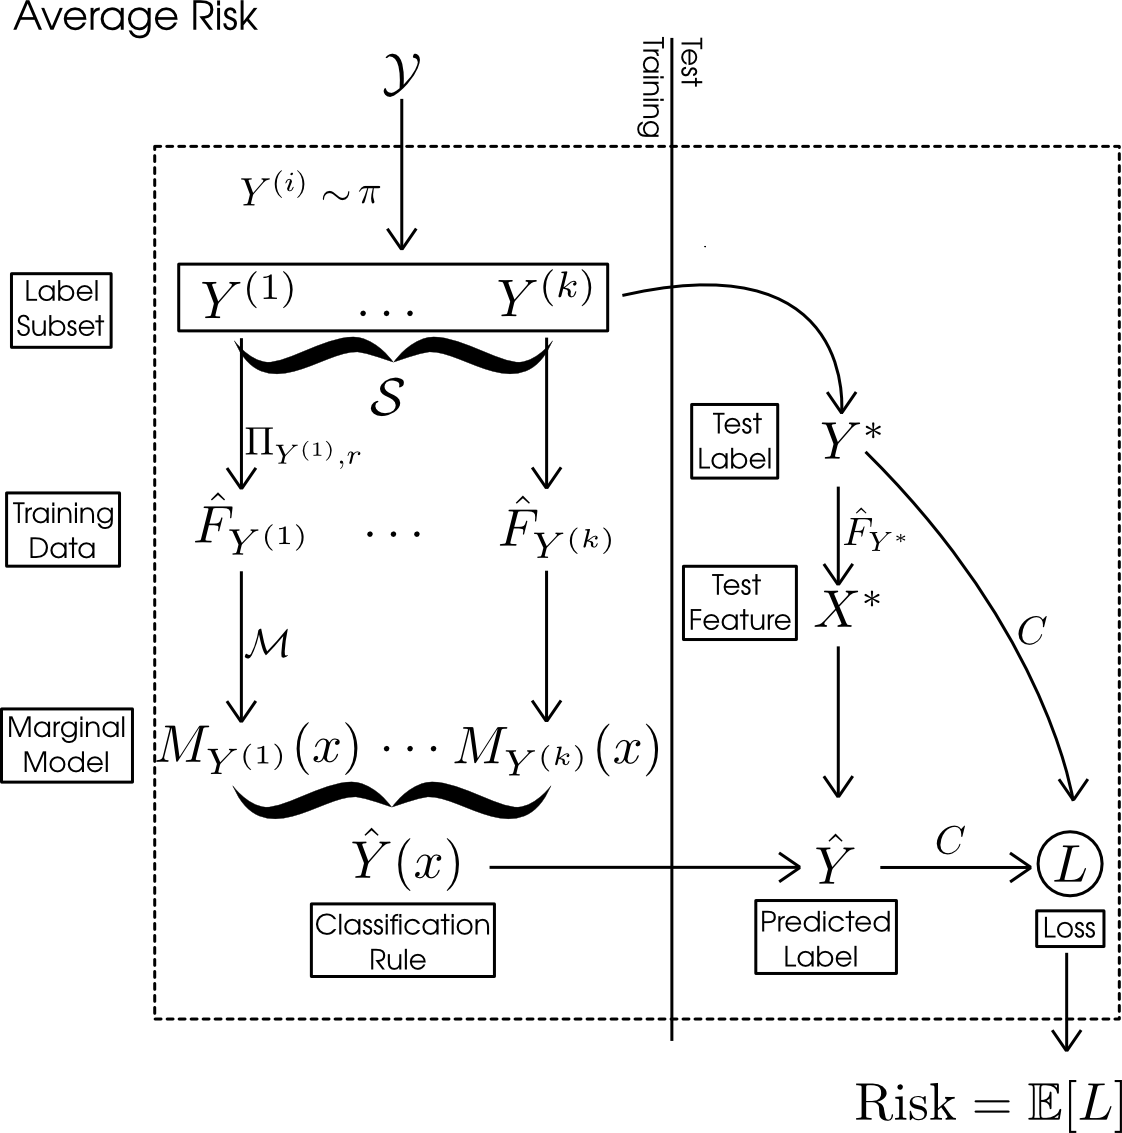
\includegraphics[scale = 0.3]{../extrapolation_figures/average_risk.png}
\caption{Average risk}\label{fig:average_risk2}
\end{figure}

As we can see from Figure \ref{fig:average_risk2}, the average risk is obtained by averaging
over four randomizations:
\begin{enumerate}
\item[A1.] Drawing the label subset $\mathcal{S}$.
\item[A2.] Drawing the training dataset.
\item[A3.] Drawing $Y^*$ uniformly at random from $\mathcal{S}$.
\item[A4.] Drawing $X^*$ from $F_{X^*}$.
\end{enumerate}

For the sake of developing a better intuition of the average risk, it
is helpful to define a random variable called the \emph{loss}, which
is the cost incurred by a single test instance.  The loss is
determined by quantities from all four randomization steps: the label
subset $\mathcal{S} = \{Y^{(1)},\hdots, Y^{(k)}\}$, the training
samples $\hat{F}_{Y^{(1)}},\hdots, \hat{F}_{Y^{(k)}}$, and the test
point $(X^*, Y^*)$.  Formally, we write
\[
L = C(\mathcal{F}(\{\hat{F}_y\}_{y \in \mathcal{S}})(X^*), Y^*).
\]
Now note that the $k$-class, $r$-repeat average risk is the expected loss,
\begin{equation}\label{eq:avrisk_EL}
\text{AvRisk}_{k, r, \nu}(\mathcal{F}) = \E[L] = \E[C(\mathcal{F}(\{\hat{F}_y\}_{y \in \mathcal{S}})(X^*), Y^*)].
\end{equation}
where the expectation is taken over the joint distribution of all the
quantities $\{Y^{(1)},\hdots,
Y^{(k)}, \hat{F}_{Y^{(1)}},\hdots, \hat{F}_{Y^{(k)}}, (X^*, Y^*)\}$.

Our strategy is to analyze the average risk \eqref{eq:avrisk_EL} by
means of \emph{conditioning on} the true label and its training
sample, $(y^*, \hat{F}_{y^*})$, and the test feature $x^*$
while \emph{averaging} over all the other random variables.  Define
the \emph{conditional average risk} $\text{CondRisk}_k((y^*, \hat{F}_{y^*}), x^*)$ as
\[
\text{CondRisk}_k((y^*, \hat{F}_{y^*}), x^*) = \E[L|Y^*=y^*, X^* = x^*, \hat{F}_{Y^*} = \hat{F}_{y^*}].
\]
Figure \ref{fig:conditional_risk} illustrates the variables which are
fixed under conditioning and the variables which are randomized.
Compare to figure \ref{fig:average_risk}.

Without loss of generality, we can write the label subset $\mathcal{S}
= \{Y^*, Y^{(1)},\hdots, Y^{(k-1)}\}$.  Note that due to independence,
$Y^{(1)},\hdots, Y^{(k-1)}$ are still i.i.d. from $\pi$ even
conditioning on $Y^* = y^*.$ Therefore, the conditional risk can be
obtained via the following alternative order of randomizations:
\begin{enumerate}
\item[C0.] 
Fix $y^*, \hat{F}_y^*,$ and $x^*$.  Note that $M_{y^*}(x^*)
= \mathcal{M}(\hat{F}_{y^*})(x^*)$ is also fixed.
\item[C1.]
Draw the \emph{incorrect labels} $Y^{(1)},\hdots, Y^{(k)}$ i.i.d. from
$\pi$.  (Note that $Y^{(i)} \neq y^*$ with probability 1 due to the
continuity assumptions on $\mathcal{Y}$ and $\pi$.)
\item[C2.]
Draw the training samples for the incorrect labels
$\hat{F}_{Y^{(1)}},\hdots, \hat{F}_{Y^{(k-1)}}$.  This determines
\[
\hat{Y} = \argmax_{y \in \mathcal{S}} M_y(x^*)
\]
and hence
\[
L = C(\hat{Y}, y^*).
\]
\end{enumerate}
Compared to four randomization steps for the average risk, we have
essentially conditioned on steps A3 and A4 and randomized over steps
A1 and A2.

\begin{figure}[h]
\centering
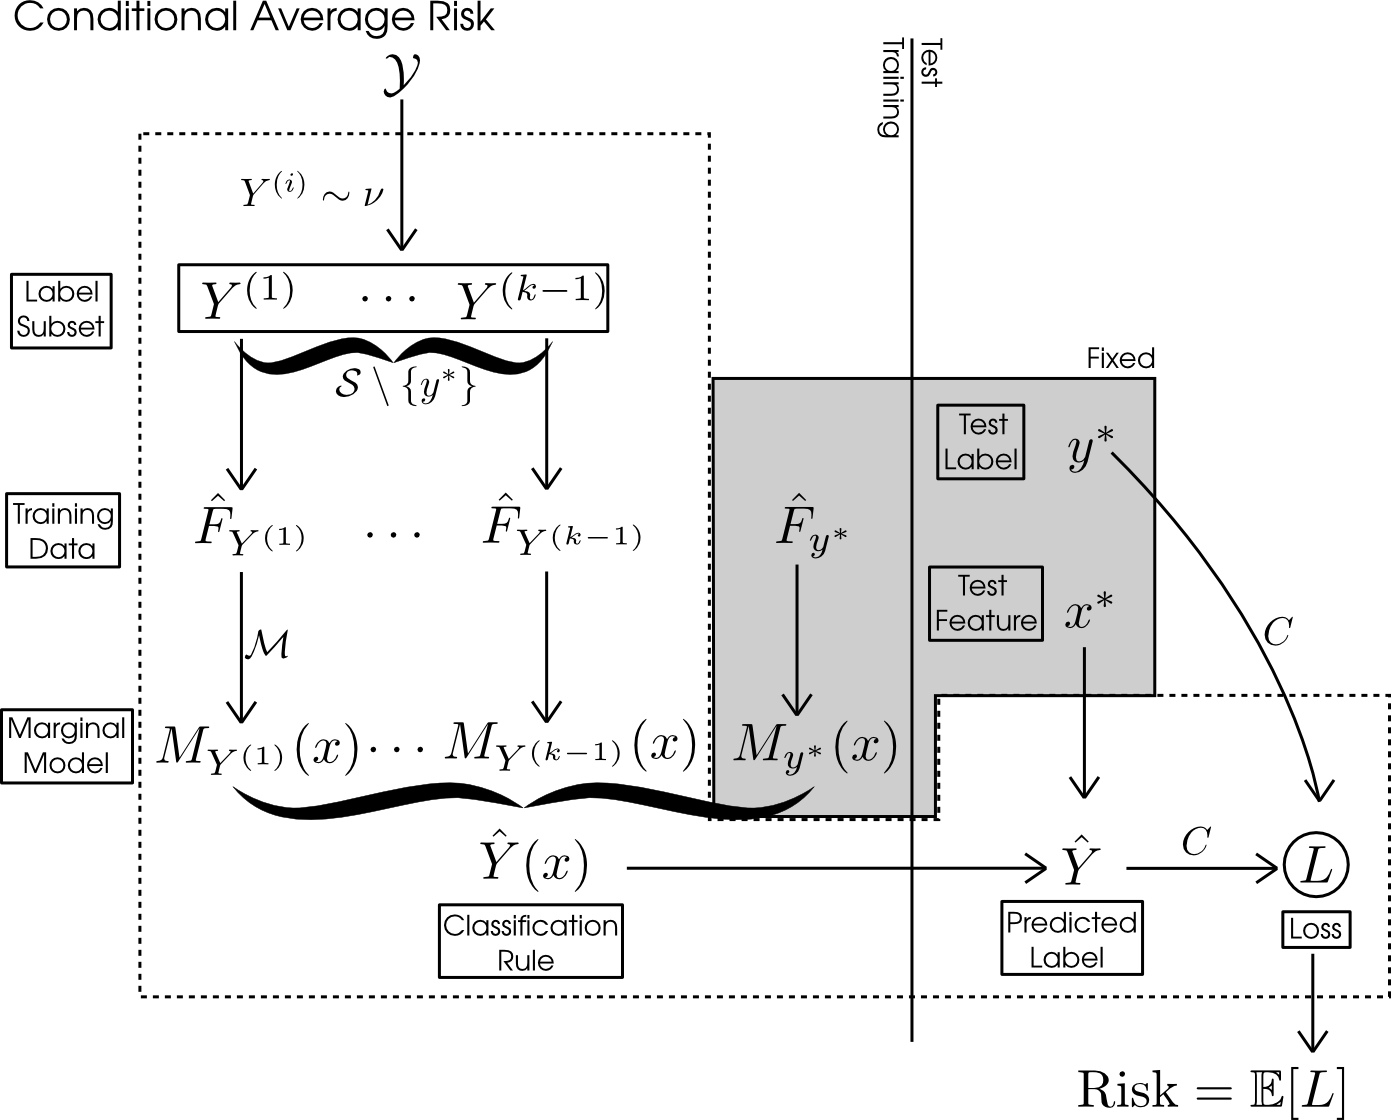
\includegraphics[scale = 0.3]{../extrapolation_figures/conditional_risk.png}
\caption{Conditional average risk}\label{fig:conditional_risk}
\end{figure}

Now, in order to analyze the $k$-class behavior of the conditional
average risk, we begin by considering the \emph{two-class} situation.

In the two-class situation, we have a true label $y^*$ and one
incorrect label, $Y$.  Define the \emph{U-function} $U_{x^*}(y^*,
\hat{F}_{y^*})$ as the \emph{probability of correct classification} in
the two-class case.  The classification is correct if the margin
$M_{y^*}(x^*)$ is greater than the margin $M_Y(x^*)$, and incorrect
otherwise.  Since we are fixing $x^*$ and $(y^*, \hat{F}_{y^*})$, the
probability of correct classification is obtained by taking an
expectation:
\begin{align}\label{eq:U_function}
U_{x^*}(y^*, \hat{F}_{y^*}) &= \Pr[M_{y^*}(x^*) > \mathcal{M}(\hat{F}_Y)(x^*)]
\\&= \int_{\mathcal{Y}} 
I\{
M_{y^*}(x^*) > \mathcal{M}(\hat{F}_{y})(x)
\}
d\Pi_{y, r}(\hat{F}_y)
d\pi(y).
\end{align}
See also figure \ref{fig:U_function} for an graphical illustration of
the definition.

\begin{figure}[h]
\centering
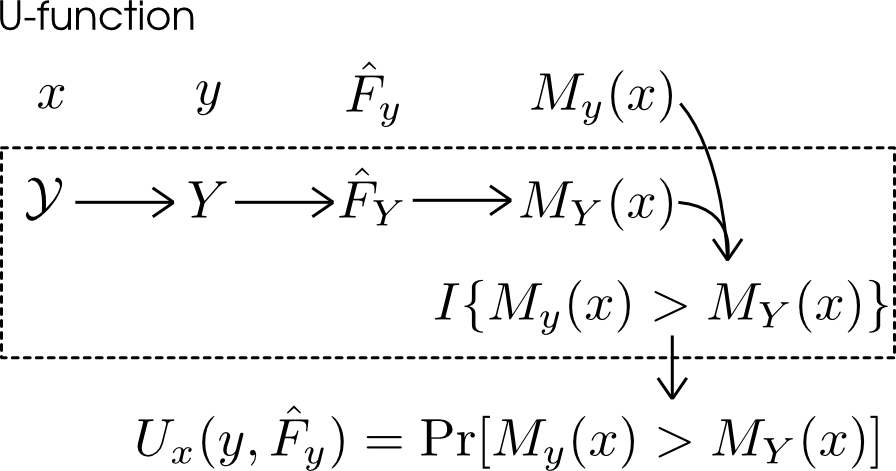
\includegraphics[scale = 0.4]{../extrapolation_figures/U_function.png}
\caption{U-functions}\label{fig:U_function}
\end{figure}

An important property of the U-function, and the basis for its name,
is that the random variable $U_x(Y, \hat{F}_Y)$ for $Y \sim \pi$ and
$\hat{F}_Y \sim \Pi_{Y, r}$ is uniformly distributed for all
$x \in \mathcal{X}$.  This is proved in Lemma \ref{lemma:U_function}
in the appendix.

Now, we will see how the U-function allows us to understand the
$k$-class case.  Suppose we have true label $y^*$ and incorrect labels
$Y^{(1)},\hdots, Y^{(k-1)}$.  Note that the U-function
$U_{x^*}(y, \hat{F}_y)$ is monotonic in $M_y(x^*)$.  Therefore,
\[
\hat{Y} = \argmax_{y \in \mathcal{S}} M_y(x^*) = \argmax_{y \in \mathcal{S}} U_{x^*}(y, \hat{F}_y).
\]
Therefore, we have a correct classification if and only if the U-function value for the correct label
is greater than the maximum U-function values for the incorrect labels:
\[
\Pr[\hat{Y} = y^*] = \Pr[U_{x^*}(y^*, \hat{F}_{y^*}) > \max_{i=1}^{k-1} U_{x^*}(Y^{(i)}, \hat{F}_{Y^{(i)}})] =  \Pr[u^* > U_{max}].
\]
where $u^* = U_{x^*}(y^*, \hat{F}_{y^*})$ and $U_{max, k-1}
= \max_{i=1}^{k-1} U_{x^*}(Y^{(i)}, \hat{F}_{Y^{(i)}})$.  But now,
observe that we know the distribution of $U_{max, k-1}$!  Since
$U_{x^*}(Y^{(i)}, \hat{F}_{Y^{(i)}})$ are i.i.d. uniform, we know that
\begin{equation}\label{eq:umax_beta}
U_{max, k-1} \sim \text{Beta}(k-1, 1). 
\end{equation}
We now have the insights needed to analyze the simplest special case: zero-one loss.
\newline

\noindent \emph{Special case: 0-1 loss}.
For zero-one loss, which is $C(y, y') = I\{y = y'\}$, we have $L=1$ if
and only if $U_{max} > u^*$ and $L=0$ otherwise.  Therefore, the
conditional average risk is
\[
\text{CondRisk}_k((y^*, \hat{F}_{y^*}), x^*) = \Pr[U_{max} > u^*] = \int_{u^*}^1 (k-1) u^{k-2} du.
\]
Now the average risk can be obtained by integrating over the distribution of $U^* = U_{x^*}(y^*, \hat{F}_{y^*})$.
We have
\begin{align*}
\text{AvRisk}_k &= \E[ \int_{U^*}^1 (k-1) u^{k-2} du] 
\\&= \E[\int_0^1 I\{u \geq U^*\} (k-1) u^{k-2} du ]
\\&= (k-1) \int_0^1 \Pr[U^* \leq u] u^{k-2} du.
\end{align*}
Or equivalently,
\[
\text{AvRisk}_{k, r, \nu}((y^*, \hat{F}_{y^*}), x^*) = (k-1) \int \bar{D}(u) u^{k-2} du.
\]
where $\bar{D}(u)$ denote the cumulative distribution function of $U^*$ on $[0,1]$:
\[
\bar{D}(u) = \Pr[U_{x^*}(y^*, \hat{F}_{y^*}) \leq u].
\]
We have expressed the average risk expressed as a weighted integral of
a certain function $\bar{D}(u)$ defined on $u \in [0,1]$.  We have
clearly isolated the part of the average risk which is independent of
$k$--the univariate function $\bar{D}(u)$, and the part which is
dependent on $k$--which is the density of $U_{max}$.

In section \ref{sec:extrapolation_estimation}, we will develop
estimators of $\bar{D}(u)$ in order to estimate the $k$-class average
risk.  But now let us return to the general case.
\newline

\noindent \emph{General loss functions.}
The case for general cost functions is somewhat more complicated,
since knowledge of $U_{max}$ is not sufficient to determine $L$.  In
short, this is because $U_{max}$ by itself is insufficient to
determine $\hat{Y}$, and therefore $L=C(\hat{Y}, y^*)$.  However, we
can resolve this issue by noting that for the purposes of computing
the expected loss, it suffices to have the \emph{conditional
distribution} of $\hat{Y}$ given $U_{max}$.  Even though $U_{max}$
does not deterministically map onto a unique $\hat{Y}$, it determines
a conditional distribution of $\hat{Y}$ which allows us to compute
$\E[L|U_{max}, x^*, y^*, \hat{F}_{y^*}]$.

Now, a key fact is that the conditional distribution of $\hat{Y}$
given $U_{max}$ \emph{does not depend} on $k$.  To see this fact,
suppose without loss of generality that $\hat{Y} = Y^{(k-1)}.$ Then
the joint density of $Y^{(1)},\hdots, Y^{(k-1)}$ given $U_{max} =
u$ can be written
\[
p(y^{(1)},\hdots, y^{(k-1)}) \propto 
\pi(y^{(k-1)})\frac{d}{dt}\Pr[U_{x^*}(y^{(k-1)}, \hat{F}_{y^{(k-1)}}) \leq t]|_{t=u}
\prod_{i=1}^{k-2}\pi(y^{(i)})\Pr[U_{x^*}(y^{(k-1)}, \hat{F}_{y^{(k-1)}}) < u].
\}
\]
up to a normalizing constant.  Note that the term
$\frac{d}{dt}\Pr[U_{x^*}(y^{(k-1)}, \hat{F}_{y^{(k-1)}}) \leq t]$ is the
density of the random variable
$U_{x^*}(Y^{(k-1)}, \hat{F}_{Y^{(k-1)}})$. From the density, we can see
that $Y^{(1)},\hdots, Y^{(k-1)}$ are conditionally independent given
$U_{max} = u$, hence the marginal density of $\hat{Y}=Y^{(k-1)}$ can
be written
\[
p(\hat{y}) \propto \pi(\hat{y})\frac{d}{dt}\Pr[U_{x^*}(y^{(k-1)}, \hat{F}_{y^{(k-1)}}) \leq t]|_{t=u}.
\]

The only property of the conditional distribution of $\hat{Y}|U_{max} = u$ that is needed is
the expectation of $L = C(\hat{Y}, y^*)$.  Therefore, define the \emph{conditional expected loss} $D((y^*, \hat{F}_{y^*}), x^*, u)$ by
\begin{equation}\label{eq:Kfunc}
D((y^*, \hat{F}_{y^*}), x^*, u) = \begin{cases} 0 \text{ if } u < u^*\\
\E[C(\hat{Y}, y^*)|U_{max} = u, x^*, y^*, \hat{F}_{y^*}] \text{ otherwise.}
\end{cases}
\end{equation}
We have the two cases $u < u^*$ and $u > u^*$ since when $U_{max} <
u^*$, the correct label is chosen and the loss is zero.  Otherwise, an
incorrect label is chosen, and the expected loss must be calculated
using the conditional distribution of $\hat{Y}$.

Again, since the conditional distribution of $\hat{Y}|U_{max}, x^*,
(y^*, \hat{F}_{y^*})$ is independent of $k$, the conditional cost
function is also independent of $k$.

With the conditional cost function and the distribution of $U_{max}$ both in hand, we can compute the average conditional risk
\[
\text{CondRisk}_k((y^*, \hat{F}_{y^*}), x^*) = (k-1) \int D((y^*,\hat{F}_{y^*}), x^*, u) u^{k-2} du.
\]
Now the average risk can be obtained by integrating over $(Y^*, \hat{F}_{Y^*}),$ and $X^*$.
\[
\text{AvRisk}_{k, r} = (k-1) \int \bar{D}(u) u^{k-2} du.
\]
where
\begin{equation}\label{eq:Kbar}
\bar{D}(u) = \int D((y^*,\hat{F}_{y^*}), x^*, u) \pi(y^*)dy dF_{y^*}(x^*) d\Pi_{y^*, r}(\hat{F}_{y^*}).
\end{equation}


This is the key result behind our estimation method, which was stated in theorem \ref{theorem:avrisk_identity}. 
The proof is given in the appendix.

Having this theoretical result allows us to understand how the
expected $k$-class risk scales with $k$ in problems where all the
relevant densities are known.  However, applying this result in
practice to estimate $\text{Average Risk}_k$ requires some means of
estimating the unknown function $\bar{D}$--which we discuss in the
following.

\section{Estimation}\label{sec:extrapolation_estimation}

Now we address the problem of estimating $\text{AvRisk}_{k_2,
r_{train}}$ from data.  As we have seen from
Theorem \ref{theorem:avrisk_identity}, the $k$-class average risk of
a marginal classifier $\mathcal{M}$ is a functional of a object called
$\bar{D}(u),$ which depends marginal model $\mathcal{M}$ of the
classifier, the joint distribution of labels $Y$ and features $X$ when
$Y$ is drawn from the sampling density $\nu$.

Therefore, the strategy we take is to attempt to estimate $\bar{D}$
for then given classification model, and then plug in our estimate of
$\bar{D}$ into the integral \eqref{eq:avrisk_identity} to obtain an
estimate of $\text{AvRisk}_{k_2, r_{train}}$.

Having decided to estimate $\bar{D}$, there is then the question of
what kind of model we should assume for $\bar{D}$.  While a
nonparametric approach may be ideal, for the case of general loss
functions we will adopt a parametric model: that is the subject of
this section.

Let us assume the linear model
\begin{equation}\label{eq:linearKu}
\bar{D}(u) = \sum_{\ell = 1}^m \beta_\ell h_\ell(u),
\end{equation}
where $h_\ell(u)$ are known basis functions, and $\beta$ are the model
parameters to be estimated. We can obtain \emph{unbiased} estimation
of $\text{AvRisk}_{k_2, r_{train}}$ via the unbiased estimates of
$k$-class average risk obtained from \eqref{eq:avtestrisk}.

If we plug in the assumed linear model \eqref{eq:linearKu} into the
identity \eqref{eq:avrisk_identity}, then we get
\begin{align}
\text{AvRisk}_{k, r_{train}} &= (k-2)\int \bar{D}(u) u^{k-2} du
\\&= (k-2)\int_0^1 \sum_{\ell = 1}^m \beta_\ell h_\ell(u) u^{k-2} du
\\&= \sum_{\ell = 1}^m \beta_\ell H_{\ell,k} \label{eq:avrisk_linear}
\end{align}
where
\begin{equation}
H_{\ell,k} = (k-2) \int_0^1 h_\ell(u) u^{k-2} du.
\end{equation}
The constants $H_{\ell, k}$ are moments of the basis function
$h_\ell$: hence we call this method the \emph{moment method.}  Note
that $H_{\ell, k}$ can be precomputed numerically for any $k \geq 2$.


Now, since the $\text{AvTestRisk}_k$ are unbiased estimates of
$\text{AvRisk}_{k, r_{train}}$, this implies that the regression
estimate
\[
\hat{\beta} = \argmin_\beta \sum_{k=2}^{k_1} w_k \left(\text{AvTestRisk}_k - \sum_{\ell=1}^m \beta_\ell H_{\ell, k}\right)^2
\]
is unbiased for $\beta$, under any choice of positive weights $w_k$.
The estimate of $\text{AvRisk}_{k_2,r_{train}}$ is similarly obtained
from \eqref{eq:avrisk_linear}, via
\begin{equation}\label{eq:avrisk_hat}
\widehat{\text{AvRisk}_{k_2,r_{train}}} = \sum_{\ell=1}^m \hat{\beta}_\ell H_{\ell, k_2}.
\end{equation}

\subsection{Large-Sample Theory}

How good are the estimated average risks \eqref{eq:avrisk_hat}?  Let
us investigate the accuracy of the estimates in the limit where
$k_1 \to \infty$, first in the case where the
model \eqref{eq:linearKu} is correctly specified, and then considering
possible model misspecification.

If we fix the number of classes $k_2$ which defines the estimation
target, then we need not use the estimator \eqref{eq:avrisk_hat},
since once $k_1 > k_2$, we can use the $\text{AvTestRisk}_{k_2}$ as an
estimator instead, which can easily be shown to a have a convergence
rate of $O(1/\sqrt{k_1})$ to the true average risk.  Therefore, if we
want to quantify the performance of the regression-based
estimator \eqref{eq:avrisk_hat}, it does not make sense to look at
asymptotic settings where $k_2$ is fixed.  One approach is to specify
a setting where $k_2$ changes as a function of $k_1$.  However, the
approach we will take is to look at the minimax error: that is, to
look at the maximum discrepancy between the estimate and the true
average risk over all $k_2$ simultaneously.  The performance criterion
is the minimax error, defined
\begin{equation}\label{eq:minimax_error}
\text{MinimaxError} = \sup_{k_2 > 2} |\widehat{\text{AvRisk}_{k_2,r_{train}}} - \text{AvRisk}_{k_2,r_{train}}|.
\end{equation}

\noindent\emph{Well-specified case.}

Let us first assume that the parametric model \eqref{eq:linearKu} is correct. Then
\[
\text{AvRisk}_{k_2,r_{train}} = \sum_{\ell=1}^m \beta_\ell H_{\ell, k_2} = \langle \vec{H}_{k_2}, \beta \rangle
\]
where $\vec{H}_{k_2} = (H_{\ell, k_2})_{\ell=1}^m$.
Then, we get
\[
\text{MinimaxError} = \sup_{k_2 > 2} |\langle \vec{H}_{k_2}, \beta - \hat{\beta}\rangle|.
\]
If we assume that all the basis functions $h_\ell(u)$ are bounded by a
common constant $M$, then it follows that $H_\ell, k$ are also bounded by the same constant $M$,
and we have
\[
\text{MinimaxError} \leq M ||\beta - \hat{\beta}||_1 \leq M \sqrt{m}||\beta - \hat{\beta}||_2
\]

Therefore, any convergence rate we can establish for $\hat{\beta}$ is
inherited by the minimax error.  Meanwhile, we can show that choosing
$k_0$ sufficiently large that $(\vec{H}_2,\hdots,\vec{H}_{k_0})$ is
full-rank, and setting weights $w_k = I\{k \leq k_0\}$, then the
resulting $\hat{\beta}$ converges to the true $\beta$ at the usual
$O(1/\sqrt{n})$ rate.  We state the result in the following theorem.

\begin{theorem}
Consider a sequence of problems where the model $\mathcal{M}$,
$r_{train}$, $r_{test}$, joint distribution
$\{F_y\}_{y \in \mathcal{Y}}$, and class sampling distribution $\eta$
are fixed as $k_1 \to \infty$.  Further assume that the function
$\bar{D}(u)$ defined by $\{F_y\}_{y \in \mathcal{Y}}$, $\eta$, and
$\mathcal{M}$ satisfies
\[
\bar{D}(u) = \sum_{\ell = 1}^m \beta_\ell h_\ell(u)
\]
for some basis functions $h_\ell(u)$.
%and that those basis functions satisfy
%\[
%\max_{\ell=1}^m ||h_\ell(u)||_\infty < M
%\]
%for some constant $M < \infty$.
Let $k_0$ be an integer sufficiently large so that
\[
\text{Rank}(\vec{H}_2,\hdots,\vec{H}_{k_0}) = m.
\]
Then, defining
\[
\hat{\beta} = \argmin_\beta \sum_{k=2}^{k_0} \left(\text{AvTestRisk}_k - \sum_{\ell=1}^m \beta_\ell H_{\ell, k}\right)^2
\]
there exists some constant $C < \infty$ such that
\[
\lim_{k_1 \to \infty} \sqrt{k_1}||\hat{\beta}-\beta||_2 = C.
\]
\end{theorem}

\textbf{Proof.}
Note that the statistics $\text{AvTestRisk}_k$ are U-statistics of the
$k_1$ pairs of test and training samples.  Therefore, by Hoeffding
1948, it follows that
$(\text{AvTestRisk}_2,\hdots, \text{AvTestRisk}_{k_0})$ is
asymptotically normal with covariance satisfying
\[
\lim_{k_1 \to \infty} k_1 \Cov(\text{AvTestRisk}_2,\hdots, \text{AvTestRisk}_{k_0}) = \Sigma,
\]
for some positive semidefinite matrix $\Sigma$.  Defining $\bH$ to be
the matrix with rows $\vec{H}_2,\hdots,\vec{H}_{k_0}$, this then
implies that
\[
\lim_{k_1 \to \infty} k_1 \Cov(\hat{\beta}) = (\bH^T \bH)^{-1} \bH^T \Sigma \bH (\bH^T \bH)^{-1}.
\]
It follows that defining
\[
C = \sqrt{\text{tr} (\bH^T \bH)^{-1} \bH^T \Sigma \bH (\bH^T \bH)^{-1}}
\]
we have
\[
\lim_{k_1 \to \infty} \sqrt{k_1}||\hat{\beta}-\beta||_2 = C.
\]
$\Box$.

\noindent\emph{Misspecified case.}

Now consider the more realistic setting where the
model \eqref{eq:linearKu} is misspecified.  We quantify the degree of
misspecification by the $\ell_\infty$ error on [0,1].  Define
\[
\delta = \inf_{\beta} \|\bar{D}(u) - \sum_{\ell = 1}^m \beta_\ell h_\ell(u)\|_\infty,
\]
and let $\tilde{\beta}$ be the coefficients $\beta$ which attain the infimum,
with $\tilde{D}(u) = \sum_{\ell = 1}^m \tilde{\beta}_\ell h_\ell(u)$.
To deal with this case, refer to the theory in section \ref{sec:misspecifiedOLS}.
For each $u = [0,1]$, find a matrix $A(u)$ such that (i) the first column equals
\[
A_1(u) = (h_1(u),\hdots, h_m(u))
\]
and that (ii) the rest of the columns are orthogonal to the first,
and (iii) $A(u)$ is full-rank.
Then define $Z(u) = X A(u)$,
and consider the column vector
\[
Z_{1|-1}(u) = (I - P_{Z_{-1}}) Z_1(u).
\]
It can be shown that $Z_{1|-1}(u)$ is well-defined, regardless of how
$A(u)$ is chosen.  Then, by the theory in section \ref{sec:misspecifiedOLS},
the extra bias due to approximation error for predicting $\hat{D}(u)$
is given by
\[
\text{Bias}^2(u) = \frac{||Z_{1|-1}(u)||_1^2}{||Z_{1|-1}(u)||_2^4}.
\]
Define the maximum bias as
\[
\text{Bias}^2_{max} = \sup_{ u \in [0,1]} \text{Bias}^2(u).
\]
From the analysis of the well-specified case, we know that the
variance component of the prediction risk decreases at order $O(1/k)$.
Therefore, the misspecified minimax error is of order
\[
\text{MinimaxError} = O(1/\sqrt{k}) + \text{Bias}^2_{max}.
\]


\section{Examples}\label{sec:extrapolation_example}

